\documentclass{beamer}
\beamertemplatenavigationsymbolsempty
\usecolortheme{beaver}
\setbeamertemplate{blocks}[rounded=true, shadow=true]
\setbeamertemplate{footline}[page number]
%
\usepackage[utf8]{inputenc}
\usepackage[english]{babel}
\usepackage{amssymb,amsfonts,amsmath,mathtext}
\usepackage{subfig}
\usepackage[all]{xy} % xy package for diagrams
\usepackage{array}
\usepackage{multicol}% many columns in slide
\usepackage{hyperref}% urls
\usepackage{hhline}%tables
% Your figures are here:
\graphicspath{ {fig/} {../fig/} }

%----------------------------------------------------------------------------------------------------------
\title[\hbox to 56mm{Influence of hyperparameters}]{Influence of hyperparameters on aggregating predictions of infinite number of experts}
\author[N.\,P.~Ivkin]{Sergey Kunin-Bogoiavlenskii}
\institute{Moscow Institute of Physics and Technology}
\date{\footnotesize
\par\smallskip\emph{Course:} My first scientific paper\par (Strijov's practice)/Group 125 %821, 813
\par\smallskip\emph{Expert:} R.\,D.~Zukhba
\par\smallskip\emph{Consultant:} A.\,V.~Zukhba
\par\bigskip\small 2024}

%----------------------------------------------------------------------------------------------------------
\begin{document}
%%----------------------------------------------------------------------------------------------------------
%\begin{frame}
%\thispagestyle{empty}
%\maketitle
%\end{frame}
%%-----------------------------------------------------------------------------------------------------
%\begin{frame}{Goal of research}
%..
%\end{frame}
%%-----------------------------------------------------------------------------------------------------
\begin{frame}{Influence of hyperparameters on aggregating predictions of infinite number of experts}

%Please comment all slides but this one if you make the One-slide talk.

\begin{columns}[c]
\column{0.6\textwidth}
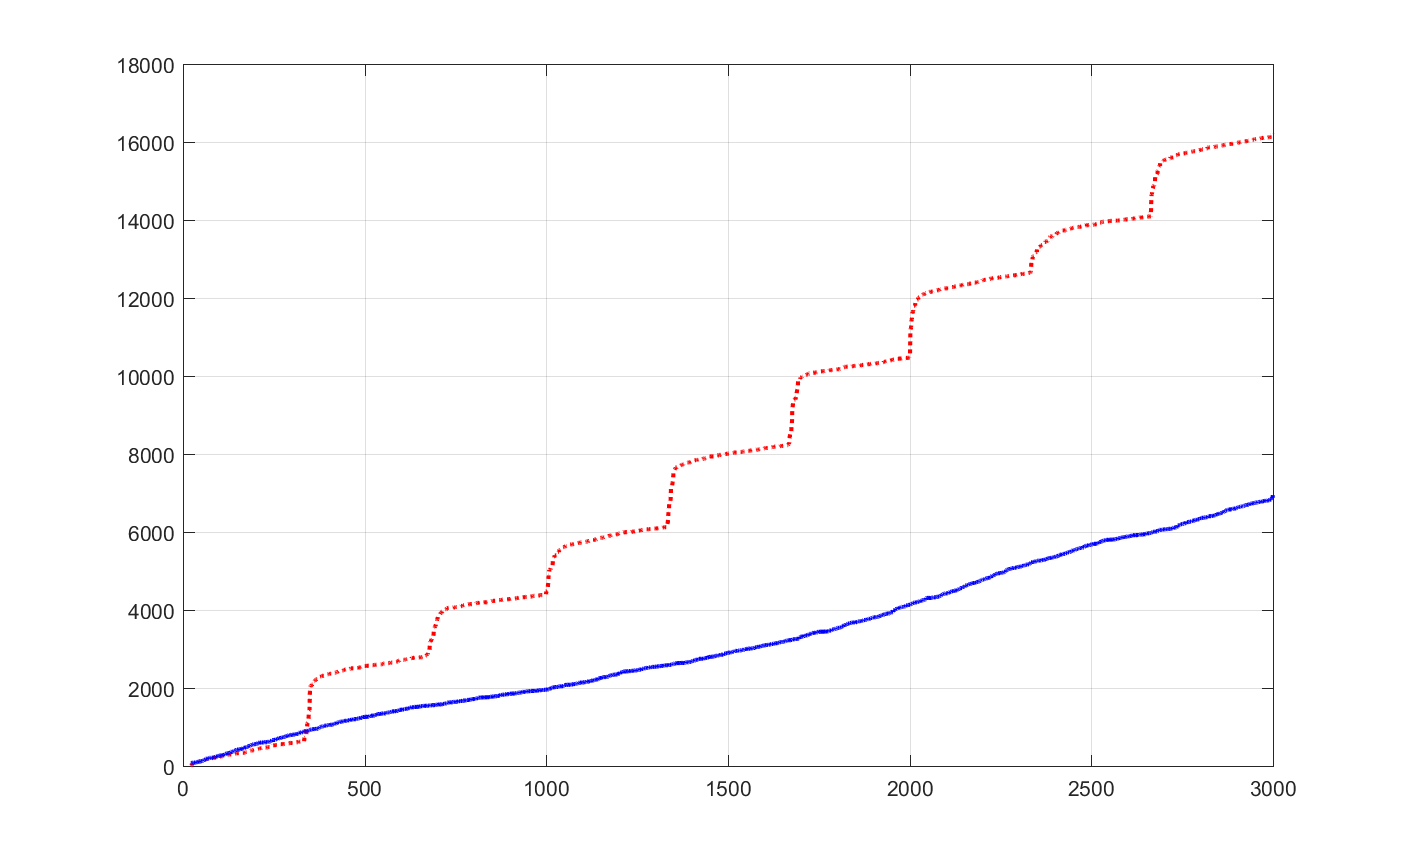
\includegraphics[width=1.0\textwidth]{ErrorFunction}
  
\column{0.6\textwidth}
    \begin{itemize}
    \item Time series generator implementation 
    \item Aggregating forecasting model implementation
    \item Conduction of experiments with various hyperparameters of the algorithm
    \end{itemize}
\end{columns}

\bigskip
\textbf{Keywords}: \emph{online learning; aggregating algorithm; prediction with experts’ advice; Fixed Share, Mixing Past Posteriors (MPP)}
\end{frame}


%%----------------------------------------------------------------------------------------------------------
%\begin{frame}{Problem statement}
%..
%\end{frame}
%%----------------------------------------------------------------------------------------------------------
%\begin{frame}{Solution}
%\begin{columns}[c]
%\column{0.6\textwidth}
%    Column 1
%\column{0.4\textwidth}
%    Column 2
%\end{columns}
%\end{frame}
%%----------------------------------------------------------------------------------------------------------
%\begin{frame}{Computational experiment}
%..
%\end{frame}
%%----------------------------------------------------------------------------------------------------------
%\begin{frame}{Conclusion}
%    \begin{block}{Forecast with hierarchical aggregation of}
%    \begin{itemize}
%        \item types of freight in
%        \item stations, regions, and roads,
%        \item for a day, week, month, and quarter.
%    \end{itemize}
%    \end{block}
%\end{frame}
%%----------------------------------------------------------------------------------------------------------
\end{document} 